\documentclass[a4paper,12pt,twoside]{article}	% debut d'un fichier latex standard

\usepackage{graphicx}	% pour l'inclusion de figures en eps,pdf,jpg
\usepackage{amsmath}	% quelques symboles mathematiques en plus
\usepackage{amssymb}
\usepackage{mathrsfs}
%\usepackage{psfrag}

\usepackage{listings}

\usepackage{mathenv}
\usepackage[british,UKenglish,USenglish,english,american]{babel}	
% \usepackage[francais]{babel}	% le tout en langue francaise
% \usepackage[latin1]{inputenc}	% on peut ecrire directement les caracteres avec l'accent(L/W)
\usepackage[colorlinks,bookmarks=false,linkcolor=blue,urlcolor=blue]{hyperref}	% pour l'inclusion de links dans le document 

\paperheight=297mm
\paperwidth=210mm

\setlength{\textheight}{235mm}
\setlength{\topmargin}{-1.2cm} % pour centrer la page verticalement -1.2
%\setlength{\footskip}{5mm}
\setlength{\textwidth}{15cm}
\setlength{\oddsidemargin}{0.2cm}
\setlength{\evensidemargin}{0.56cm}

\pagestyle{plain}

% quelques abreviations utiles
\def \be {\begin{equation}}
\def \ee {\end{equation}}
\def \bs {\begin{equation} \left\{  \begin{aligned}}
\def \es {\end{aligned} \right. \end{equation}}
\def \dd  {{\rm d}}
\def \un {\,\,\mathrm}


\newcommand{\mail}[1]{{\href{mailto:#1}{#1}}}
\newcommand{\ftplink}[1]{{\href{ftp://#1}{#1}}}


% ======= Le document commence ici ======
\begin{document}

% Le titre, l'auteur et la date
\title{Optical tweezer}
\date{\today}
\author{
	% Laurent \bsc{Rohrbasser}\\{\small \mail{laurent.rohrbasser@epfl.ch}} \and 
	% Tim \bsc{Tuuva}\\{\small \mail{tim.tuuva@epfl.ch}}
	Laurent Rohrbasser\\{\small \mail{laurent.rohrbasser@epfl.ch}} \and 
	Tim Tuuva\\{\small \mail{tim.tuuva@epfl.ch}}
	}
\maketitle

\tableofcontents % Table des matieres

% Quelques options pour les espacements entre lignes, l'identation 
% des nouveaux paragraphes, et l'espacement entre paragraphes
\baselineskip=16pt
\parindent=15pt
\parskip=5pt

% \section{Abstract}
\begin{abstract}

This document will show the results got on an implementation of the lowcost optical tweezer decribed in the paper called "Inexpensive optical tweezers for undergraduate laboratories". The goal is to see how well that experiments works on simple shapes such as tiny dielectric spheres in water by looking at their position through time while trapped and not trapped.

\end{abstract}

\section{Introduction}
An optical tweezer is a focused beam of light which can hold microscopic particles in three dimensions. It was first reported ine 1970 by Arthur Ashkin in Bell labs. Optical tweezers are useful in many areas, as in biology for instance. This tool can apply an attractive or a repulsive force on living cells or any microscopic dieletric objects. Therefore, this experiment aims to introduce ourselves to optical tweezers and the optical trapping force, mean squares displacement and (un)confined Browmian motions analysis.


\section{Theory}
There are different phenomena that applies, depending on the size of the dieletric objects, to explain the trapping force.
If the objects is much more smaller than the laser wavelenght we use the electric dipole model.
If the objects is much more bigger than the laser wavelenght we explain the trapping by the refracting force and the momentum conservation.
This experiment uses a red HeNe laser light with a $658 nm$ wavelenght and the smallest objects size is $0.5\micro m$, %TODO CHECK WAVELENGTH
therefore we will focus on the optic approach.

The individual rays of light (from the laser) are refracted at the interface of the dieletric, when they enter and leave it.
Since light is associated with a momentum, one can notice that its momentum change when its direction change.
By applying the third law of Newton and the conservation of momentum, the momentum of light is transfered to the particle when the ray is refracted.


\begin{figure}[h]
	\begin{center}
	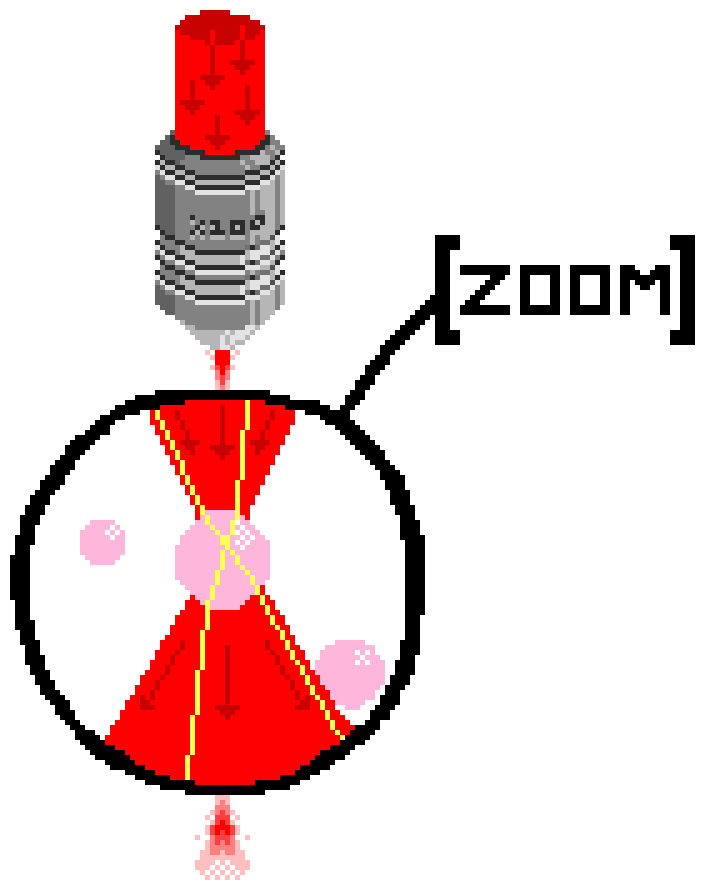
\includegraphics[width=0.5\linewidth,angle=0]{./figures/lazor_zoom}
	\caption{TODO} \label{fig:theory}
	\end{center}
\end{figure}

\section{Dispositif}
There are two main parts to build an optical tweezer:
\begin{itemize}
	\item Microscope
	\item Laser system
\end{itemize}

\subsection{Microscope}
It is made of an objective and an ocular lens. A lamp enlights the sample placed in the focal plane of the objective lens which enlarged the observed object. A filter is placed between the objective and the lens to filter out the laser beam reflected from the sample plate. Finally, the ocular lens focus the objective image into the CCD camera which shows us the image on a monitor screen.

\subsection{Laser system}
The laser is sent into the microscope objective using mirrors and a dichoirc mirror. It reflects the laser beam on one direction and let it pass on the other direction.
Initially, the laser is colimated, but since it is too small one should enlarged it, using 2 lens placed in each other focal plane, thus to create a telescope. Therefore, the laser is enlarged and slightly diverging when arriving into the objective. This particular configuration helps to the trapping force effect.

\begin{figure}[h]
	\begin{center}
		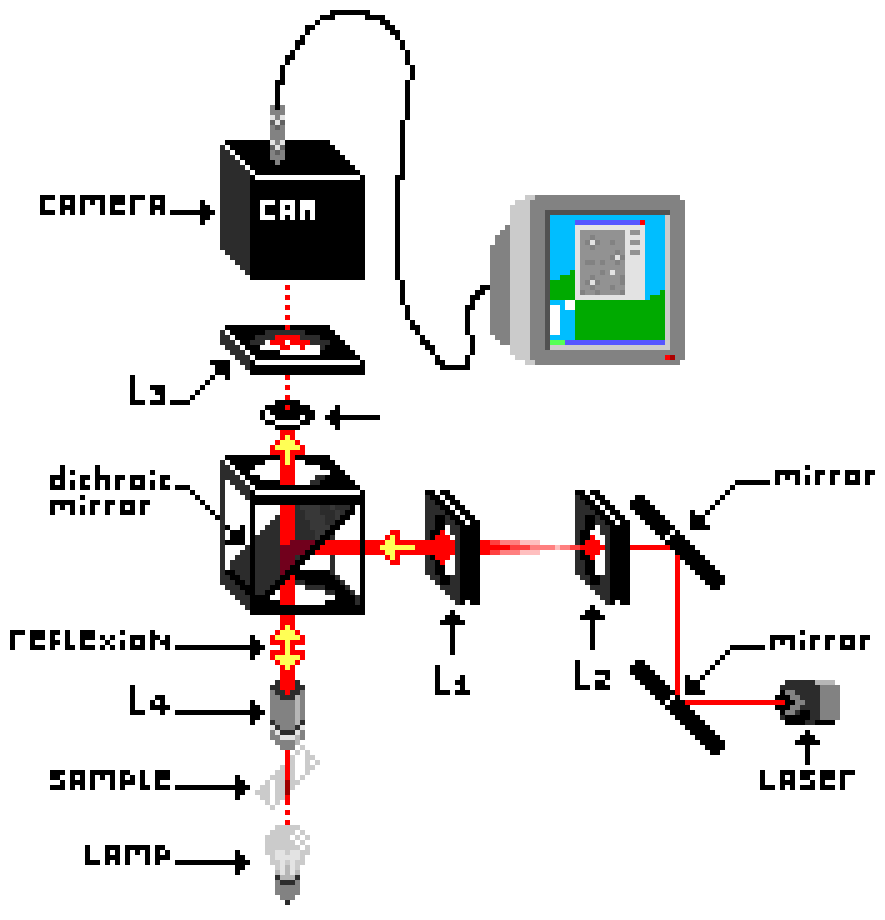
\includegraphics[width=0.6\linewidth,angle=0]{./figures/montage_1}
		\caption{Optical tweezer setup schema.} \label{fig:dispositif}
	\end{center}
\end{figure}

\section{Results}

The microscope part did work well. After many observations on serval samples with different concentrations, it was possible to get a $XXXXXXX $x zoom with a clear image when the focus was correct. All particles were distinguishable and it was observed that if a partcle moved on z, the focus was easly lost but that did happen slowly, so it was not a big problem to collect data. It had been a delicate task to find the best lighting so that the algorithm of the given software (MOSAIC in imageJ) can detect some particles (the particle had to appear darker or brighter than everything else, the ring shape was not the optimal input).

ILLUSTRATION DETECTION PARTICULE RING -> GROS CACA

ILLUSTRATION DETECTION PARTICULE POINT -> TRAJECTOIRE

c'est quoi qu'on a vu ?

- le trap selon x y : OK

- le trap selon z : pas OK (decrire ce qui s'est passe)

\section{Analyse et Discussion}

- expliquer les calculs

- le trap selon x y : montrer que ca marche

- le trap selon z : expliquer

le plus important!!!

\section{Conclusion}

un bref résumé de la manipulation, revenir sur les buts, une analyse avec plus de recul de l'expérience et ses résultats

description du but du TP

description du dispositif experimental

Résumé (abstract)
Introduction (et background théorique)
Dispositif
Résultats
Bibliographie





\end{document} %%%% THE END %%%%


